\subsection{Feasibility Study}
\begin{itemize}
\item Technical Feasibility As this whole project is based on C and C++ as programming language, technical feasibility of this project revolves around the technical boundaries of the C++. As we need parser for our project, so we are also using Flex and Bison for this.
These languages are perfect to design the software under this project.\\
\item Economic Feasibility Almost all the softwares used in this project are Open source and the software released under this project are Open source too and are released under GNU GPLv3 (General Public Licence). So this project is fully economic feasible.\\
\item Operational Feasibility This project is also operationalally feasible which not only saves time but also saves money as mast the work done by this software.
\end{itemize}

\subsection{System Design}
Based on the user requirements and the detailed analysis of a new system, the new system must be designed. This is the phase of system designing normally, the design proceeds
in two stages:-\\
\begin{itemize}
\item Preliminary or general design.
\item Structure or detailed design.
\end{itemize}
{\bf Preliminary or general design}\\
In the preliminary or general design, the features of the new system are specified.\\\\
{\bf Structure or Detailed design}\\
In the detailed design stage, computer oriented work begins in earnest. Input, output and processing specifications are drawn up in detail.\\\\
{\bf There are several tools and techniques used for designing}\\
\begin{itemize}
\item Data flow diagram (DFDs).
\item ER Diagram.
\end{itemize}
Design is the first step into the development phase for any engineered product or system. Design is a creative process. A good design is the key to effective system. The term
"design" is defined as "the process of applying various techniques and principles for the purpose of defining a process or a system in sufficient detail to permit its physical realization". It may be defined as a process of applying various techniques and principles for the purpose of defining a device, a process or a system in sufficient detail to permit its physical realization. Software design is the technical kernel of the software engineering
process and is applied regardless of the development paradigm that is used. The system design develops the architectural detail required to build a system or product. As in the case of any systematic approach, this software too has undergone the best possible design phase fine tuning all efficiency, performance and accuracy levels.
% \subsection{Implementation Of Project}
% \begin{figure}[h!]
% \centering
% 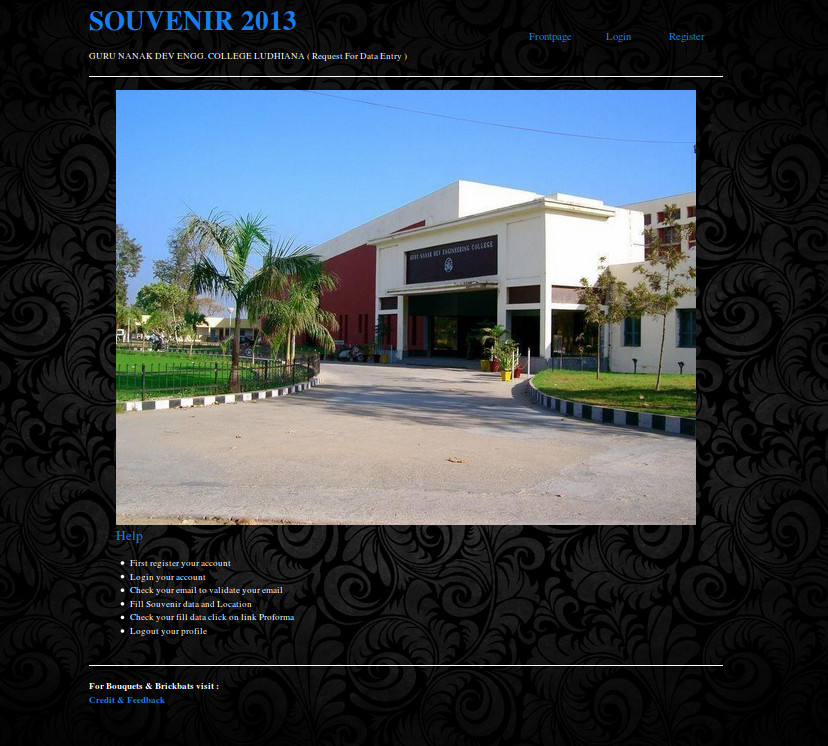
\includegraphics[width=0.6\textwidth]{images/fp.png}
% \caption{Souvenir}
% \end{figure}
% Yaadein software woks in following different steps
% \begin{itemize}
% \item Fetching of data from the database.
% \item Typesetting of data.
% \item Including graphics.
% \item Creating DVI file.
% \item Creating post script file.
% \item Creating pdf file.
% \item Imposition of the pdf.
% \item Color separation of the pdf(Optional)
% \end{itemize}
% Now let us discuss above points in detail
% \subsubsection{Fetching of data from the database}
% As for making SOUVENIR all the information required like student personal information, contact details,etc. were needed to be stored somewhere so phpMyAdmin was used
% fo this purpose.\\
% phpMyAdmin is a free software tool written in PHP intended to handle the\\
% \image{0.5}{images/phpadmin.png}{phpMyAdmin logo}
% administration of MySQL over the World Wide Web. phpMyAdmin supports a wide range of operations with MySQL. The most frequently used operations are supported by the user interface (managing databases, tables, fields, relations, indexes, users, permissions, etc), while you still have the ability to directly execute any SQL statement.\\
% phpMyAdmin had already become one of the most popular PHP applications and MySQL administration tools, with a large community of users and contributors. In order to co-
% ordinate the growing number of patches, a group of three developers registered The phpMyAdmin Project at SourceForge.net and took over the development in 2001.
% Features.\\\\
% \begin{itemize}
% \item Web interface.
% \item MySQL database management.
% \item Import data from CSV and SQL.
% \item Export data to various formats: CSV, SQL, XML, PDF (via the TCPDF library), ISO/IEC 26300 - OpenDocument Text and Spreadsheet, Word, Excel, \LaTeX{} and others.
% \item Administering multiple servers.
% \item Creating PDF graphics of the database layout.
% \item Creating complex queries using Query-by-example (QBE).
% \item Searching globally in a database or a subset of it.
% \item Transforming stored data into any format using a set of predefined functions, like displaying BLOB-data as image or download-link.
% \item Active query monitor (Processes).
% \end{itemize}
% Fetching data from the database and this is done through php programmming. PHP initially makes a connection with database before fetching teh data.
% \begin{verbatim}
% <?php
% $conn = mysql_connect("localhost", $userName, $passWord);
% mysql_select_db($DB);
% ?>
% \end{verbatim}
% \subsubsection{Typesetting of data}
% Second step after fetching data was indeed to fit that at right place for which \LaTeX{} was used. \LaTeX{} is Type Setting editor. Lots of things were tried to make the look of the document better from tables to frame alast psframebox were used to set the data.
% \begin{verbatim}
% \psframebox*[par]{stuff}
% \end{verbatim}
% A simple frame (perhaps with rounded corners) is drawn using
% \begin{verbatim}
% \psframe
% \end{verbatim}
% The * option is of particular interest. It generates a solid frame whose color is fillcolor (rather than linecolor, as with the closed graphics objects). Recall that the default value of fillcolor is white, and so this has the effect of blotting out whatever is behind the
% box. Small example\\
% \image{0.4}{images/record.png}{Record of students}\\
% \begin{verbatim}
% \rput(1.2;35){\psframebox*{\small\$9.0M}}
% \uput{2.2}[45](0,0){Oreos}
% \rput(1.2;135){\psframebox*{\small\$16.7M}}
% \uput{2.2}[135](0,0){Heath}
% \rput(1.2;280){\psframebox*{\small\$23.1M}}
% \uput{2.2}[280](0,0){M\\&M}
% \endpspicture
% \end{verbatim}
% \subsubsection{Creating a DVI file}
% The Device independent file format (DVI) is the output file format of the TeX typesetting program, designed by David R. Fuchs in 1979.[1] Unlike the TeX markup files used to generate them, DVI files are not intended to be human-readable; they consist of binary data describing the visual layout of a document in a manner not reliant on any
% specific image format, display hardware or printer. DVI files are typically used as input to a second program (called a DVI driver) which translates DVI files to graphical data. For example, most TeX software packages include a program for previewing DVI files on a user’s computer display; this program is a driver. Drivers are also used to convert from DVI to popular page description languages (e.g. PostScript, PDF) and for printing.\\\\
% DVI differs from PostScript and PDF in that it does not support any form of font embedding. (Both PostScript and PDF formats can either embed their fonts inside the
% documents, or reference external ones.) For a DVI file to be printed or even properly previewed, the fonts it references must be already installed. Also, unlike PostScript, DVI is not a full, Turing-complete programming language, though it does use a limited sort of machine language.\\
% Command :\$ latex file name
% \subsubsection{Creating a postscript file}
% PostScript (PS) is a dynamically typed concatenative programming language created by John Warnock and Charles Geschke in 1982. PostScript is best known for its use as a
% page description language in the electronic and desktop publishing areas.\\\\
% The concepts of the PostScript language were seeded in 1976 when John Warnock was working at Evans \& Sutherland, a computer graphics company. At that time John Warnock was developing an interpreter for a large three-dimensional graphics database of New York harbor. Warnock conceived the Design System language to process the graphics.\\
% \image{0.5}{images/typesetting.png}{Type-setting using tables}\\

% Command: \$ dvips file name -o

% \subsubsection{Use In Printing}
% Prior to the introduction of PostScript, printers were designed to print character output given the texttypically in ASCIIas input. There were a number of technologies for this task, but most shared the property that the glyphs were physically difficult to change, as they were stamped onto typewriter keys, bands of metal, or optical plates.\\\\
% PostScript printing\\
% PostScript went beyond the typical printer control language and was a complete programming language of its own. Many applications can transform a document into a PostScript
% program whose execution will result in the original document. This program can be sent to an interpreter in a printer, which results in a printed document, or to one inside another application, which will display the document on-screen. Since the document-program is the same regardless of its destination, it is called device independent.\\

% \image{0.4}{images/psbox.png}{Type-setting using psframebox}

% \subsubsection{Creating a PDF file}
% Portable Document Format (PDF) is an open standard for document exchange. This file format created by Adobe Systems in 1993 is used for representing documents in a manner independent of application software, hardware, and operating systems.Each PDF file encapsulates a complete description of a fixed-layout flat document, including the text, fonts, graphics, and other information needed to display it.\\\\
% The PDF combines three technologies:\\
% \begin{itemize}
% \item A subset of the PostScript page description programming language, for generating the layout and graphics.
% \item A font-embedding/replacement system to allow fonts to travel with the documents.
% \item A structured storage system to bundle these elements and any associated content into a single file, with data compression where appropriate.
% \end{itemize}
% Command: \$ ps2pdf file name.ps\\
% \image{0.4}{images/device.png}{Device Independent File}

% \subsubsection{Imposition of the pdf}
% Imposition is one of the fundamental steps in the prepress printing process. It consists in the arrangement of the printed product’s pages on the printer’s sheet, in order to obtain faster printing, simplify binding and reduce paper waste.\\
% Correct imposition minimizes printing time by maximizing the number of pages per impression, reducing cost of press time and materials. To achieve this, the printed sheet must be filled as fully as possible.\\\\
% Below code will convert and merge two pdf files on single page eg:
% \image{0.2}{images/imp.png}{Imposition of pdf files}
% \begin{verbatim}
% \documentclass{article}
% \pdfpagewidth 283mm
% \pdfpageheight 460mm
% \usepackage[pdftex]{color,graphicx,epsfig}
% \usepackage[paperwidth=283mm,paperheight=460mm,left=0cm,top=0cm,bottom=0cm,right=0cm]{geometry}
% \usepackage[final]{pdfpages}   %for including pdf files 
% \begin{document}
% \includepdf[pages=-, signature=8,landscape]{cover8.pdf}  %Cover8 folder contains all pdf files without imposition
% \end{document}
% \end{verbatim}
% After merging two pdf pages on single page, next we have to do imposition of pages in such a way that after folding that pdf sheet front-inside,front-outside,back-inside and back-outside goes to their respective position.
% \begin{verbatim}
% \documentclass{article}
% \pdfpagewidth 460mm
% \pdfpageheight 566mm
% \usepackage[pdftex]{color,graphicx,epsfig}
% \usepackage[paperwidth=460mm,paperheight=566mm,left=0mm,top=0mm,bottom=0mm,right=0mm]{geometry}    
% \usepackage[final]{pdfpages}
% \begin{document}
% 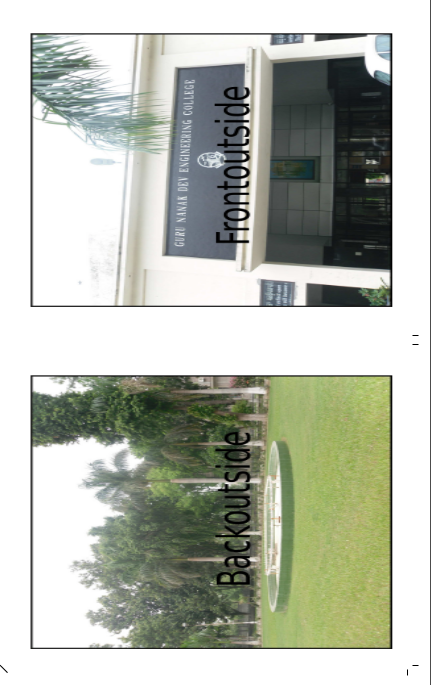
\includepdf[pages=-, signature=4,landscape]{imp.pdf}
% \end{document}
% \end{verbatim}
% This will typeset the pages on their respective position eg:\\
% \image{0.3}{images/imp2.png}{Final Imposition}
% \newpage
% \subsubsection{Color separation of the pdf}
% Color printing or Colour printing is the reproduction of an image or text in color (as opposed to simpler black and white or monochrome printing). Any natural scene or color photograph can be optically and physiologically dissected into three primary colors, red, green and blue, roughly equal amounts of which give rise to the perception of white, and different proportions of which give rise to the visual sensations of all other colors. The additive combination of any two primary colors in roughly equal proportion gives rise to the perception of a secondary color. For example, red and green yields yellow, red and blue yields magenta (a purple hue), and green and blue yield cyan (a turquoise hue). Only yellow is counter-intuitive. Yellow, cyan and magenta are merely the "basic" secondary colors: unequal mixtures of the primaries give rise to perception of many other colors all of which may be considered "tertiary."
% \subsubsection{RGB}
% The RGB color model is an additive color model in which red, green, and blue light are added together in various ways to reproduce a broad array of colors. The name of the model comes from the initials of the three additive primary colors, red, green, and blue.\\\\
% The main purpose of the RGB color model is for the sensing, representation, and display of images in electronic systems, such as televisions and computers, though it has also been used in conventional photography. Before the electronic age, the RGB color model already had a solid theory behind it, based in human perception of colors.\\
% \image{0.3}{images/rgb.png}{RGB color}

% \subsubsection{CMYK}
% The CMYK color model (process color, four color) is a subtractive color model, used in color printing, and is also used to describe the printing process itself. CMYK refers to the four inks used in some color printing: cyan, magenta, yellow, and key (black). Though it varies by print house, press operator, press manufacturer, and press run, ink is typically applied in the order of the abbreviation.The "K" in CMYK stands for key because in four-color printing, cyan, magenta, and yellow printing plates are carefully keyed, or aligned, with the key of the black key plate.\\
% The CMYK model works by partially or entirely masking colors on a lighter, usually white, background. The ink reduces the light that would otherwise be reflected. Such a model is called subtractive because inks "subtract" brightness from white.In additive color models such as RGB, white is the "additive" combination of all primary colored lights, while black is the absence of light. In the CMYK model, it is the opposite: white is the natural color of the paper or other background, while black results from a full combination of colored inks.
% \image{0.3}{images/cmyk.png}{CMYK color}

% \subsubsection{RGB to CMYK}
% \image{0.7}{images/rgbcmyk.jpeg}{RGB and CMYK difference}
% \hspace{-1.8em} A comparison of RGB and CMYK color spaces. The image demonstrates the difference between the RGB and CMYK color gamuts. The CMYK color gamut is much smaller than the RGB color gamut, thus the CMYK colors look muted. If you were to print the image on a CMYK device (an offset press or maybe even a ink jet printer) the two sides would likely look much more similar, since the combination of cyan, yellow, magenta and black cannot reproduce the range (gamut) of color that a computer monitor displays. This is a constant issue for those who work in print production. Clients produce bright and colorful images on their computers and are disappointed to see them look muted in print.\\\\
% How to convert RGB to CMYK?\\\\
% First we need imagemagick. Install it using following command:\\\\
% \$ sudo apt-get install imagemagick\\\\
% Following commands convert the rgb pdf file  to cmyk\\
% 1. Check whether the final.pdf is rgb or cmyk\\
% \$ identify -verbose ‘final.pdf’\\\\
% It displayes the many properties. Check colorspace: rgb /cmyk\\
% \image{0.2}{images/r1.png}{RGB Check}\\
% If it displayes cmyk, then its ok. Otherwise need to convert into cmyk\\\\
% 2. To convert rbg to cmyk use following command:\\\\
% \$ gs -dSAFER -dBATCH -dNOPAUSE -dNOCACHE -sDEVICE=pdfwrite -sColorConversionStrategy=CMYK -dProcessColorModel=/DeviceCMYK -sOutputFile=output.pdf input.pdf\\
% \begin{verbatim}
% NOTE:- input.pdf = your_file_name.pdf
% output.pdf = output_pdf_file.pdf
% It displays the following output:
% \end{verbatim}
% \image{0.2}{images/r2.png}{RBG to CMYK page convertion}
% Replace the input.pdf with your test pdf file\\
% 3. Now again check the properties of pdf file by following command:\\
% \$ identify -verbose 'test.pdf'\\
% It displays the following output:\\
% \image{0.2}{images/r3.png}{CMYK converted pages}\\

% \subsection{Evaluation and Maintenance}
% Implementation is the process of having systems personnel check out and put new equipment into use, train users, install the new application and construct any files of data
% needed to use it. This phase is less creative than system design. Depending on the size of the organization that will be involved in using the application and the risk involved
% in its use, systems developers may choose to test the operation in only one area of the firm with only one or two persons. Sometimes, they will run both old and new system
% in parallel way to compare the results. In still other situations, system developers stop using the old system one day and start using the new one the next.\\
% Evaluation of the system is performed to identify its strengths and weaknesses. The actual evaluation can occur along any of the following dimensions:\\
% \begin{itemize}
% \item Operational Evaluation: Assessment of the manner in which the system functions, including case of use, response time, overall reliability and level of utilization.
% \item Organizational Impact: Identification and measurement of benefits to the organization in such areas as financial concerns, operational efficiency and competitive impact.
% \item User Manager Assessment: Evaluation of the attitudes of senior and user manager within the organization, as well as end-users.
% \item Development Performance: Evaluation of the development process in accordance with such yardsticks as overall development time and effort, conformance to budgets.
% \end{itemize}
% \image{0.3}{images/device_indp.png}{Device Independent File Created}
% and standards and other project management criteria.\\\\
% Maintenance is necessary to eliminate errors in the working system during its working life and to tune the system to any variations in its working environment often small system deficiencies are found as a system is brought into operations and changes are made to remove them. System planners must always plan for resource availability to carry out these maintenance functions. The importance of maintenance is to continue to bring the new system to standards.\\
% \image{0.3}{images/ps.png}{Post Script File Created}
% \newpage
% \subsection{RGB To CMYK Example :-}
% \begin{figure}[h!]
% \centering
% 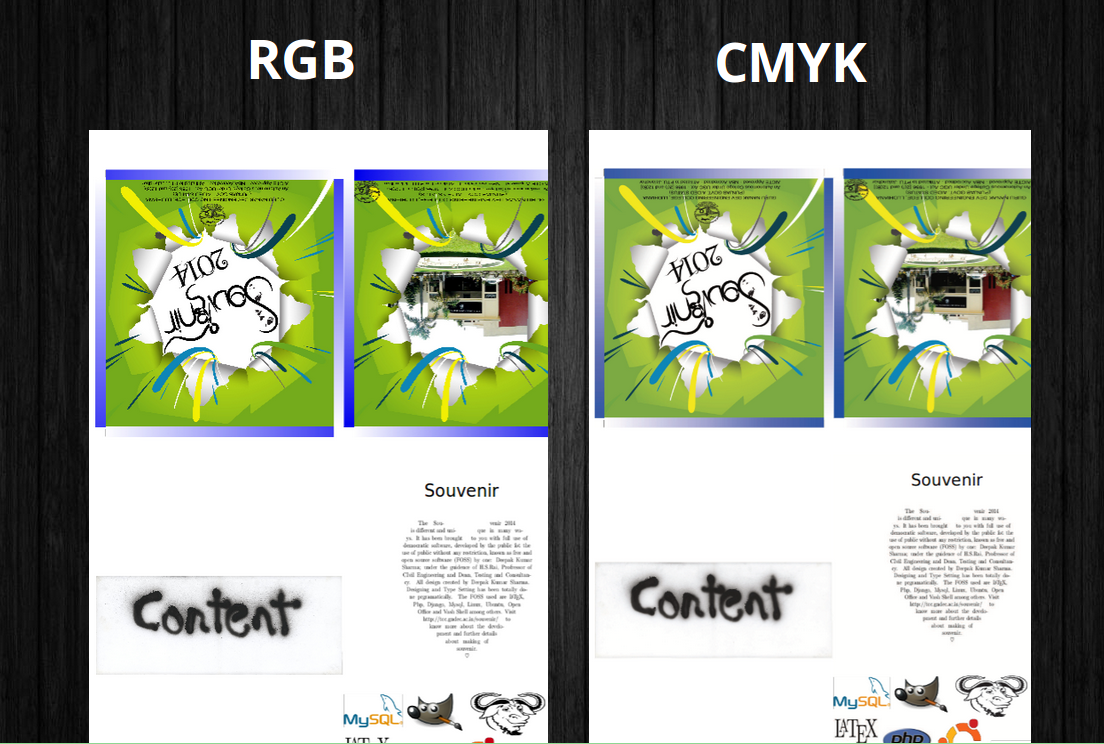
\includegraphics[width=0.8\textwidth]{images/rc.png}
% \caption{RGB To CMYK}
% \end{figure}
